\chapter{Over-Approximation and Under-Approximation}
\section{Approximation Theory}
\begin{comment}
$F = \exists x_1 \in I_1 \cdots x_n \in I_n. \bigwedge \limits_j \psi_j(x_1,\cdots,x_n)$, 
%\exists x_1 \ldots x_n. (\underbrace{\bigwedge \limits_i x_i \in I_i}_{I}) \wedge 
%                       (\underbrace{\bigwedge \limits_j \psi_j(x_1,\cdots,x_n)}_{P})
where $\psi_j(x_1,\cdots,x_n)$ is an atomic formula. 
%
$F$ is equivalnet to 
$\exists x_1 \ldots x_n. (\bigwedge \limits_i x_i \in I_i) \wedge (\bigwedge \limits_j \psi_j(x_1,\cdots,x_n))$, 
and we call $\bigwedge \limits_i x_i \in I_i$ {\em interval constraints}, and 
we refer $\bigwedge \limits_j \psi_j(x_1,\cdots,x_n)$ by $\psi(x_1,\cdots,x_n)$. 
Initially, interval constraints have a form of the conjunction $\bigwedge \limits_i x_i \in I_i$, 
and later by refinement, $x_i \in I_i$ is decomposed into a clause $\bigvee_j x_i \in I_{i_j}$, 
which makes a CNF. 

As an SMT (SAT modulo theory) problem, 
boolean variables are assigned to each $x_i \in I_{i_j}$, 
and truth assignments is produced by a SAT solver, 
which are proved or disproved by a background theory $T$ whether it satisfies $\psi(x_1,\cdots,x_n)$. 

As notational convention, $m$ (the lower case) denotes 
a variable assignments on $x_i$'s, and 
$M$ (the upper case) denotes a truth assignment on $x_i \in I_{i_j}$'s. 
We write $m \in M$ when an instance $m = \{ x_i \leftarrow c_i \}$ satisfies 
all $c_i \in I_{i_j}$ that are assigned true by $M$. 

We assume {\em very lazy theory learning}~\cite{dpll}, and 
a backend theory $T$ is applied only for a full truth assignment $M$. 
%We regard $M$ as a conjunction $\bigwedge \limits_i x_i \in I_{i_j}$. 
\begin{itemize}
\item If an instance $m$ satisfies $\psi(x_1,\cdots,x_n)$, we denote $m \models_T \psi(x_1,\cdots,x_n)$. 
\item If each instance $m$ with $m \in M$ satisfies $\psi(x_1,\cdots,x_n)$, 
we denote $M \models_T \psi(x_1,\cdots,x_n)$. 
\end{itemize}
\end{comment}

\begin{comment}
\begin{definition} \label{def:app}
Let $F = \exists x_1 \in I_1 \cdots x_n \in I_n. \psi(x_1,\cdots,x_n)$. 
For a truth assignment on $M$, $F$ is 
\begin{itemize}
\item $T$-valid if $M \models_T \psi(x_1,\cdots,$ $x_n)$, 
\item $T$-satisfiable ($T$-SAT) if $m \models_T \psi(x_1,\cdots,x_n)$ 
for some $m \in M$, and 
\item $T$-unsatisfiable ($T$-UNSAT) if $M \models_T \neg \psi(x_1,\cdots,x_n)$. 
\end{itemize}
If $T$ is clear from the context, we simply say valid, satisfiable, and unsatisfiable. 
\end{definition}
\end{comment}

%%%%%%%%%%%%%
\suppress{
Then, Fig. \ref{fig:T_result} illustrates Definition~\ref{def:app}. 
\begin{figure} [ht]
\centering
\begin{minipage}[b]{0.45\linewidth}
  \includegraphics[height=1.8in,width=1.9in]{T_result.eps}
\caption{Results of a target constraint $F$ in a theory $T$}
\label{fig:T_result}
\end{minipage}
\quad
\begin{minipage}[b]{0.45\linewidth}
   \includegraphics[height=2.2in,width=2.3in]{frame_app.eps}
\caption{{\bf raSAT} loop}
\label{fig:frame}
\end{minipage}
\end{figure}
}
%%%%%%%%%%%%%%%%%%%%%%%%%%%%%%%%

\begin{definition} \label{def:ApproxTheory}
Let $T, T'$ be $\Sigma$-theories and $\varphi$ be any $\Sigma$-formula. 
\begin{itemize}
\item $T'$ is an {\em over-approximation theory} (of $T$) 
iff $T'$-UNSAT of $\varphi$ implies $T$-UNSAT of $\varphi$.
\item $T'$ is an {\em under-approximation theory} (of $T$)
iff $T'$-SAT of $\varphi$ implies $T$-SAT of $\varphi$. 
\end{itemize}
\end{definition}

\begin{theorem}
If $T_O$ be an over-approximation theory of $T$, then for any $\Sigma$-formula $\varphi$: $\varphi$ is $T_O$-VALID $\implies \varphi$ is $T$-VALID.
\end{theorem}

\begin{proof}
$\varphi$ is $T_O$-VALID $\implies$ $\neg\varphi$ is $T_O$-UNSAT (Lemma \ref{lemma:theory-valid-unsat}) $\implies \neg\varphi$ is $T$-UNSAT (Definition \ref{def:ApproxTheory}) $\implies \varphi$ is T-VALID (Lemma \ref{lemma:theory-valid-unsat})
\end{proof}

%Note that $O.T$-valid can be regarded as $U.T$, since $O.T$-valid implies $T$-valid, thus $T$-SAT. 
A typical ICP applies $O.T$ only as an interval arithmetic. 
Later in Section~\ref{sec:approximation}, we will instantiate interval arithmetic as $O.T$. 
Adding to $O.T$-valid, {\bf raSAT} introduce testing as $U.T$ to accelerate SAT detection. 

\section{Interval Arithmetic as an Over-Approximation Theory}
A model $M^p_{IA} = (U^p_{IA}, I^p_{IA})$ over intervals contains a set of all intervals $U^p_{IA} = \{[l, h] | l, h \in \mathbb{R} \text{ and } l <= h\}$ and a map $I^p_{IA}$ that satisfies the following conditions.
\begin{enumerate}
\item $I^p_{IA}(Real) = U^p_{IA}$
\item $\forall p \in P^p$; $I^p_{IA}(p)= U^p_{IA} \times U^p_{IA} \mapsto U^p_{IA}$ where $I^p_{IA}(p)(i_1, i_2) = i_1 \; p_{IA} \; i_2$. The definition of $ p_{IA}$ is as follow:
\begin{itemize}
\item $[l_1, h_1] \succ_{IA} [l_2,  h_2] = true \iff l_1 > h_2$
\item $[l_1, h_1] \succ_{IA} [l_2,  h_2] = false \iff h_1 \le l_2$
\item $[l_1, h_1] \prec_{IA} [l_2,  h_2] = true \iff h_1 < l_2$
\item $[l_1, h_1] \prec_{IA} [l_2,  h_2] = false \iff l_1 \ge h_2$
\item $i_1 \succeq_{IA} i_2 = \neg(i_1 \prec_{IA} i_2)$
\item $i_1 \preceq_{IA} i_2 = \neg(i_1 \succ_{IA} i_2)$
\item $i_1 \approx_{IA} i_2 = i_1 \succeq_{IA} i_2 \wedge i_1 \preceq_{IA} i_2$
\item $i_1 \not\approx_{IA} i_2 = \neg(i_1 \approx_{IA} i_2)$
\end{itemize}
\item $\forall f \in F^p \setminus \{\mathbf{1}\}$; $I^p_{IA}(f) = U^p_{IA} \times U^p_{IA} \mapsto U^p_{IA}$ such that $ I^p_{IA}(f)(i_1, i_2)= i_1 \; f_{IA} \; i_2$ where $f_{IA}$ satisfies the following properties:
\begin{itemize}
\item $i_1 \oplus_{IA} i_2 \supseteq \{r_1 + r_2| r_1 \in i_1 \text{ and } r_2 \in i_2\}$.
\item $i_1 \ominus_{IA} i_2 \supseteq \{r_1 - r_2| r_1 \in i_1 \text{ and } r_2 \in i_2\}$.
\item $i_1 \otimes_{IA} i_2 \supseteq \{r_1 * r_2| r_1 \in i_1 \text{ and } r_2 \in i_2\}$.
\end{itemize}
\item $I^p_{IA}(\mathbf{1}) = [1,1]$
\item $\forall v \in V$; $I^p_{IA} \in U^p_{IA}$
\end{enumerate}
Theory $T^p_{IA} = \{M^p_{IA}| M^p_{IA} \text{ is a model over intervals}\}$. Each model differs to another by the mapping from variables to intervals. As a consequence, one assignment from variables to intervals can be used to describe an model. We denote $\Pi^p_{IA}$ as the model represented by $\Pi = \{x \in [l, h] | v \in V\}$. 

\begin{lemma} \label{lemma:IA-R-OP}
$\forall i_1, i_2 \in U^p_{IA}; \forall r_1 \in i_2, r_2 \in i_2; \forall p \in P^p (i_1 \; p_{IA} \; i_2 = false \implies \neg(r_1 \; p_\mathbb{R} \; r_2))$
\end{lemma}

\begin{proof}
Let $i_1 = [l_1, h_1]$ and $i_2 = [l_2, h_2]$ where $l_1 \le h_1$ and $l_2 \le h_2$. We have: 
\begin{itemize}
\item $r_1 \in i_1 \implies l_1 \le r_1 \le h_1$. 
\item $r_2 \in i_2 \implies l_2 \le r_2 \le h_2$. 
\end{itemize}
Suppose  that $i_1 \; p_{IA} \; i_2 = false$, we need to show $\neg(r_1 \; p_\mathbb{R} \; r_2)$ by considering all the possible cases of $p$:
\begin{enumerate}
\item If $p$ is $\succ$, the we have $[l_1, h_1] \succ_{IA} [l_2, h_2] = false \implies h_1 \le l_2 \implies r_1 \le r_2$ (because $r_1 \le h_1$ and $l_2 \le r_2$) $\implies \neg(r_1 > r2) \implies \neg(r_1 \succ_\mathbb{R} r_2)$.
\item If $p$ is $\prec$, the we have $[l_1, h_1] \prec_{IA} [l_2, h_2] = false \implies l_1 \ge h_2 \implies r_1 \ge r_2$ (because $r_1 \ge l_1$ and $r_2 \le h_2$) $\implies \neg(r_1 < r_2) \implies \neg(r_1 \prec_\mathbb{R} r_2)$.
\item If $p$ is $\succeq$, the we have $[l_1, h_1] \succeq_{IA} [l_2, h_2] = false \implies \neg ([l_1, h_1] \prec_{IA} [l_2, h_2]) = false \implies [l_1, h_1] \prec_{IA} [l_2, h_2] = true \implies h_1 < l_2 \implies r_1 < r_2$ (because $r_1 \le h_1$ and $r_2 \ge l_2$) $\implies \neg(r_1 \ge r_2) \implies \neg(r_1 \succeq_\mathbb{R} r_2)$.
\item If $p$ is $\preceq$, the we have $[l_1, h_1] \preceq_{IA} [l_2, h_2] = false \implies \neg ([l_1, h_1] \succ_{IA} [l_2, h_2]) = false \implies [l_1, h_1] \succ_{IA} [l_2, h_2] = true \implies l_1 > h	_2 \implies r_1 > r_2$ (because $r_1 \ge l_1$ and $r_2 \le h_2$) $\implies \neg(r_1 \le r_2) \implies \neg(r_1 \preceq_\mathbb{R} r_2)$.
\item If $p$ is $\approx$, the we have $i_1 \approx_{IA} i_2 = false \implies i_1 \succeq_{IA} i_2 \wedge i_1 \preceq_{IA} i_2 = false \implies i_1 \succeq_{IA} i_2 = false \text{ or } i_1 \preceq_{IA} i_2 = false \implies r_1 < r_2 \text{ or } r_1 > r_2$ (as the third and fourth case of this proof) $\implies \neg(r_1 = r_2) \implies \neg(r_1 \approx_\mathbb{R} r_2)$.
\item If $p$ is $\not\approx$, the we have $i_1 \not\approx_{IA} i_2 = false \implies \neg(i_1 \approx_{IA} i_2) = false \implies \neg(i_1 \succeq_{IA} i_2 \wedge i_1 \preceq_{IA} i_2) = false \implies \neg(i_1 \succeq_{IA} i_2) \vee \neg(i_1 \preceq_{IA} i_2) = false \implies i_1 \prec_{IA} i_2 \vee i_1 \succ_{IA} i_2 = false \implies i_1 \prec_{IA} i_2 = false \text{ and } i_1 \succ_{IA} i_2 = false \implies r_1 \ge r_2 \text{ and } r_1 \le r_2$ (as the first and second case of this proof) $\implies r_1 = r_2 \implies \neg(r_1 \not= r_2) \implies \neg(r_1 \not\approx_\mathbb{R} r_2)$.
\end{enumerate}
\end{proof}

\begin{theorem} \label{theorem:IA-OverAprox}
If $\Pi = \{v \in [l, h] | v \in V\}$ is a map from variables to intervals, then $\{\Pi^p_{IA}\}$ is an over-approximation of $\Pi^p_\mathbb{R}$.
\end{theorem}

\begin{lemma} \label{lemma:IA-OT}
$\forall t \in TERM^p \; \forall M^p_\mathbb{R} \in \Pi^p_\mathbb{R} \; t^{M^p_\mathbb{R}} \in t^{\Pi^p_{IA}}$.
\end{lemma}

\begin{proof}
Proof is done by induction on structure of term.
Let $t \in TERM^p$ and $M^p_\mathbb{R} = (\mathbb{R}, I^p_\mathbb{R}) \in \Pi^p_\mathbb{R}$
\begin{enumerate}
\item If $t = v \in V$, then $t^{M^p_\mathbb{R}} = I^p_\mathbb{R}(v) \in \Pi(v)$ because $M^p_\mathbb{R} \in \Pi^p_\mathbb{R}$. In addition, $t^{\Pi^p_{IA}} = \Pi^p_\mathbb{R}$.
\item If $t = \mathbf{1}$, then $t^{M^p_\mathbb{R}} = 1 \in [1, 1] = t^{\Pi^p_{IA}}$
\item If $t = t_1 \; f \; t_2$ for some $f \in F^p \setminus \{0, 1\}$

$t^{M^p_\mathbb{R}} = t_1^{M^p_\mathbb{R}} \; f_\mathbb{R} \; t_1^{M^p_\mathbb{R}}$

$t^{\Pi^p_{IA}} = t_1^{\Pi^p_{IA}} \; f_{IA} \; t_2^{\Pi^p_{IA}}$

By induction hypothesis, we have $t_1^{M^p_\mathbb{R}} \in t_1^{\Pi^p_{IA}}$ and $t_1^{M^p_\mathbb{R}} \in t_2^{\Pi^p_{IA}}$. In addition, due to the properties of $f_{IA}$: $t_1^{M^p_\mathbb{R}} \; f_\mathbb{R} \; t_1^{M^p_\mathbb{R}} \in t_1^{\Pi^p_{IA}} \; f_{IA} \; t_2^{\Pi^p_{IA}}$, or $t^{M^p_\mathbb{R}} \in t^{\Pi^p_{IA}}$ 
\end{enumerate}
\end{proof}

\begin{proof}
In order to prove Theorem ~\ref{theorem:IA-OverAprox}, we need to prove that $\forall \varphi^p (\varphi^p$ is $\{\Pi^p_{IA}\}$-UNSAT $\implies \varphi^p$ is $\Pi^p_\mathbb{R}$-UNSAT). 

Given an $\Sigma^p$-formula $\varphi^p$ and suppose that $\varphi^p$ is $\{\Pi^p_{IA}\}$-UNSAT.
Suppose $\varphi^p$ is not $\Pi^p_\mathbb{R}$-UNSAT, that means it is either  $\Pi^p_\mathbb{R}$-SAT or  $\Pi^p_\mathbb{R}$-VALID. In either case, there exist at least a model $M^p_\mathbb{R} \in \Pi^p_\mathbb{R}$ such that $\models_{M^p_\mathbb{R}} \varphi^p \iff (\varphi^p)^{M^p_\mathbb{R}}= true$.
\begin{enumerate}
\item If $\varphi^p = p(t_1, t_2)$ for some $p \in P^p$, then $(\varphi^p)^{M^p_\mathbb{R}}= true \implies t_1^{M^p_\mathbb{R}} \; p_\mathbb{R} \; t_2^{M^p_\mathbb{R}}$. 

On the other hand, $\varphi^p$ is $\{\Pi^p_{IA}\}$-UNSAT $\implies (\varphi^p)^{\Pi^p_{IA}} = false \implies t_1^{\Pi^p_{IA}} \; p_{IA} \; t_2^{\Pi^p_{IA}} = false$. In addition, because $t_1^{M^p_\mathbb{R}} \in t_1^{\Pi^p_{IA}}$ and $t_2^{M^p_\mathbb{R}} \in t_2^{\Pi^p_{IA}}$ (Lemma ~\ref{lemma:IA-OT}), $t_1^{\Pi^p_{IA}} \; p_{IA} \; t_2^{\Pi^p_{IA}} = false \implies \neg(t_1^{M^p_\mathbb{R}} \; p_\mathbb{R} \; t_2^{M^p_\mathbb{R}})$ (Lemma ~\ref{lemma:IA-R-OP}). This is a contradiction. As the result, $\varphi^p$ must be $\Pi^p_\mathbb{R}$-UNSAT.
\item If $\varphi^p = \varphi^p_1 \wedge \varphi^p_2$, then we have $\varphi^p$ is  $\{\Pi^p_{IA}\}$-UNSAT $\implies \not\models_{\Pi^p_{IA}}(\varphi^p_1 \wedge \varphi^p_2) \implies (\varphi^p_1 \wedge \varphi^p_2)^{\Pi^p_{IA}} = false \implies (\varphi^p_1)^{\Pi^p_{IA}} \wedge (\varphi^p_2)^{\Pi^p_{IA}} = false \implies (\varphi^p_1)^{\Pi^p_{IA}} = false$ and $(\varphi^p_2)^{\Pi^p_{IA}} = false$. By induction hypothesis, $\varphi^p_1$ and $\varphi^p_2$ are $\Pi^p_\mathbb{R}$-UNSAT $\implies \forall M^p_\mathbb{R} \in \Pi^p_\mathbb{R} \; \not\models_{M^p_{IA}} \varphi^p_1$ and $\forall M^p_\mathbb{R} \in \Pi^p_\mathbb{R} \; \not\models_{M^p_{IA}} \varphi^p_2 \implies \forall M^p_\mathbb{R} \in \Pi^p_\mathbb{R} \; \not\models_{M^p_{IA}} (\varphi^p_1 \wedge \varphi^p_2) \implies \varphi^p_1 \wedge \varphi^p_2$ is $\Pi^p_\mathbb{R}$-UNSAT.
\end{enumerate}
\end{proof}

\section{Testing as an Under-Approximation Theory}
\begin{definition}
Let $T^p \subseteq T^p_\mathbb{R}$ be a sub-theory of real numbers. Any sub-theory $T^p_T$ of $T^p$, i.e. $T^p_T \subseteq T^p$ is call a theory of testing with respect to $T^p$.
\end{definition}

\begin{theorem}
If $T^p_T$ is a theory of testing w.r.t $T^p$, $T^p_R$ is an under-approximation of $T^p$.
\end{theorem}

\begin{proof}
Let $\varphi^p$ is a $\Sigma^p$-formula and suppose it is $T^p_T$-SAT. We need to prove $\varphi^p$ is $T^p$-SAT. We have $\varphi^p$ is $T^p_T$-SAT $\implies \exists M^p \in T^p_T \; \models_{M^p} \varphi^p \implies \exists M^p \in T^p \; \models_{M^p} \varphi^p$ (because $T^p_T \subseteq T^p$) $\implies \varphi^p$ is $T^p$-SAT.
\end{proof}

Given a theory $T^p$, we randomly select a number of its models to form a theory of testing $T^p_T$ w.r.t $T^p$.

\section{raSAT loop}
\begin{grammar}
<bound\_atom> ::= <variable> $\in$ [real, real] | <variable> $\in$ (-inf, real] | <variable> $\in$ [real, inf) | <variable> $\in$ (-inf, inf)


<bound\_constraint> ::= $\bigwedge\limits_i\bigvee\limits_jbound\_atom_{ij}$
\end{grammar}
In other word, each model can be represented by an assignment of one real number to each variable. 
State of search procedure contains  $(\Pi, \varphi, \Pi^c, \varphi^V, \varphi^U)$ where 
\begin{itemize}
\item $\Pi$ is the interval constraint
\item $\varphi$ represents the polynomial constraint.
\item $\varphi^V$ contains the constraints that are valid under over-approximation.
\item $\varphi^U$ is the set of constraints which are UNKNOWN under over-approximation.
\end{itemize}
The transition rules are described in Table ~\ref{tab:transition-rules}. Figure ~\ref{fig:smt-design} illustrates the transition system. 

\begin{table*}[t]
  \centering
  \begin{tabular}{ll}
  \hline\\
  \large 
  $\frac{\Pi \models_{SAT} \bot}{(\Pi, \varphi, \emptyset, \emptyset, \emptyset) \to UNSAT}$ \tiny $\Pi$\_UNSAT \\\\
  \large 
  $\frac{\Pi \models_{SAT} \Pi^c \quad \Pi^{c'} = flattern(\Pi^c)}{(\Pi, \varphi, \emptyset, \emptyset, \emptyset) \to (\Pi, \varphi, \Pi^{c'}, \emptyset, \emptyset)}$ \tiny $\Pi$\_SAT\\\\
  \large
  $\frac{\Pi^c \not= \emptyset \quad   \varphi^V \wedge \varphi^U = \varphi \quad \varphi^V \cup \varphi^U = \emptyset \quad \varphi^V \text{ is }  \Pi^c_{IA}\text{-VALID}}{(\Pi, \varphi, \Pi^c, \emptyset, \emptyset) \to (\Pi, \varphi, \Pi^c, \varphi^V, \varphi^U)}$ \tiny IA\_SAT \\\\  
  \large 
  $\frac{\varphi^V = \varphi}{(\Pi, \varphi, \Pi^c, \varphi^V, \varphi^U) \to SAT}$ \tiny IA\_VALID \\\\
  \large 
  $\frac{\Pi^c \not= \emptyset \quad \varphi^U \not= \emptyset \quad \varphi^U \text{ is }  \Pi^c_T\text{-SAT}}{(\Pi, \varphi, \Pi^c, \varphi^V, \varphi^U) \to SAT}$ \tiny TEST\_SAT \\\\
  \large 
  $\frac{\varphi^U \text{ is }  \Pi^c_T\text{-UNSAT} \quad x_j \in var(\varphi^U) \quad (I_j = x_j \in [l_j, h_j]) \in \Pi^c \quad l_j < d \in \mathbb{R} < h_j \quad I_{j1} = x_j \in [l_j, d] \quad I_{j2} = x_j \in [d, h_j]}{(\Pi, \varphi, \Pi^c, \varphi^V, \varphi^U) \to (\Pi \wedge (\neg I_j \vee I_{j1} \vee I_{j2}) \wedge (I_j \vee \neg I_{j1}) \wedge (I_j \vee \neg I_{j2}) \wedge (\neg I_{j1} \vee \neg I_{j2}), \varphi, \emptyset, \emptyset, \emptyset)}$ \tiny REFINE \\\\
  \large 
  $\frac{\{\varphi_i| \varphi_i \wedge \varphi'_i = \varphi; \; \varphi_i \text{ is } \Pi^c_{IA}\text{-UNSAT}\} \quad var(\varphi_i) = \{x_{ij}|j=1,\cdots, m_i\} \quad (I_{ij} = x_{ij} \in [l_{ij}, h_{ij}]) \in \Pi^c}{(\Pi, \varphi, \Pi^c, \emptyset, \emptyset) \to (\Pi \wedge \bigwedge\limits_i \bigvee\limits_{j=1}^{m_i} \neg I_{ij}, \varphi, \emptyset, \emptyset, \emptyset)}$ \tiny IA\_UNSAT \\\\
  \hline\\
  \end{tabular}
  \caption{Transition rules}\label{tab:transition-rules}
\end{table*}

\section{Soundness - Completeness}
\subsection{Soundness}
\begin{theorem}
Let $(\Pi, \varphi, \Pi^c, \varphi^V, \varphi^U)$ be any state of our system, then the following properties are invariants:
\begin{enumerate}
\item $\Pi^c_\mathbb{R} \subseteq T^p_\mathbb{R}$
\item $\varphi^V$ is $\Pi^c_{R}$-VALID.
\item $\varphi^U = \emptyset \vee (\varphi = \varphi^U \wedge \varphi^V)$
\item $\varphi$ is $\Pi_\mathbb{R}$-UNSAT $\implies$ $\varphi$ is $T^p_\mathbb{R}$-UNSAT
\end{enumerate}
\end{theorem}

\begin{proof}
\begin{enumerate}
\item Easy from the definition.
\item Easy to see.
\item Easy from the transitions.
\item The proof is done inductively:
\begin{itemize}
\item Initial state: $(\bigwedge\limits_{v \in V}v \in (-\infty, +\infty), \varphi, \emptyset, \emptyset, \emptyset)$ and by definition, $((\bigwedge\limits_{v \in V}v \in (-\infty, +\infty))_\mathbb{R} = T^p_R$. Then, the invariant trivially holds.
\item Each transition is considered:
\begin{itemize}
\item For rules $\Pi$\_SAT, IA\_SAT the interval constraint $\Pi$ does not changed, so if the properties holds for the former state, it also does for the later one.
\item For REFINE transition: Denote $\Pi' = \Pi \wedge (\neg I_j \vee I_{j1} \vee I_{j2}) \wedge (I_j \vee \neg I_{j1}) \wedge (I_j \vee \neg I_{j2}) \wedge (\neg I_{j1} \vee \neg I_{j2})$. We will prove that $\varphi$ is $\Pi'_\mathbb{R}$-UNSAT $\implies \varphi$ is $\Pi_\mathbb{R}$-UNSAT. First suppose that $\varphi$ is $\Pi'_\mathbb{R}$-UNSAT. Let
\item for IA\_UNSAT transition, 
\end{itemize}
\end{itemize}
\end{enumerate}
\end{proof}

\begin{theorem}
Let $\varphi$ be the polynomial constraint to be solved. Starting with the state $(\Pi, \varphi, \emptyset, \emptyset, \emptyset)$, if our transitional system terminates and output:
\begin{itemize}
\item SAT then $\varphi$ is $T^p_\mathbb{R}$-SAT.
\item UNSAT then $\varphi$ is $T^p_\mathbb{R}$-UNSAT.
\end{itemize}
\end{theorem}

\begin{proof}
\begin{enumerate}
\item If the system output SAT, there are two possibles transition to SAT:
\begin{itemize}
\item In the case of IA\_VALID, we have $\varphi^V$ is $\Pi^c_{R}$-VALID (invariant 2) $\implies \varphi^V$ is $\Pi^c_\mathbb{R}$-SAT $\implies \varphi$ is $\Pi^c_\mathbb{R}$-SAT (because $\varphi^V = \varphi$ is the condition of this transition). In addition, following invariant 1, we have $\Pi^c_\mathbb{R} \subseteq T^p_\mathbb{R}$, then $\varphi$ is $T^p_\mathbb{R}$-SAT (Lemma ~\ref{lemma:subtheory-SAT}).
\item In the case of TEST\_SAT, $\varphi^U$ is $\Pi^c_\mathbb{R}$-SAT $\implies \exists M \in \Pi^c_\mathbb{R} \; \models_M \varphi^V$. Let $M^c_\mathbb{R} \in \Pi^c_\mathbb{R}$ such that $\models_{M^c_\mathbb{R}} \varphi^V$ which implies $(\varphi^V)^{M^c_\mathbb{R}} = true$. In addition, because $\varphi^V$ is $\Pi^c_\mathbb{R}$-VALID (invariant 2) and $M^c_\mathbb{R} \in \Pi^c_\mathbb{R}$, we have $\models_{M^c_\mathbb{R}} \varphi^U$ or $(\varphi^U)^{M^c_\mathbb{R}} = true$. Consider the evaluation of $\varphi$ under the model $M^c_\mathbb{R}$: $(\varphi)^{M^c_\mathbb{R}} = (\varphi^U \wedge \varphi^V)^{M^c_\mathbb{R}}$ (invariant 3) $= (\varphi^U)^{M^c_\mathbb{R}} \wedge (\varphi^V)^{M^c_\mathbb{R}} = true \wedge true = true \implies \models_{M^c_\mathbb{R}} \varphi \implies \varphi$ is $\Pi^c_\mathbb{R}$-SAT $\implies \varphi$ is $T^p_\mathbb{R}$-SAT (because of invariant 1 and Lemma ~\ref{lemma:IA-R-OP})
\end{itemize}
\item  If the system output UNSAT, there is only one transition of rule $\Pi$\_UNSAT. Because $\Pi \models_{SAT} \bot$, $\Pi_\mathbb{R}$ is empty (Lemma ?). As a result, $\varphi$ is $\Pi_\mathbb{R}$-UNSAT which implies that $\varphi$ is $T^p_\mathbb{R}$-UNSAT (invariant 4).
\end{enumerate}
\end{proof}

\subsection{Completeness}

\begin{comment}
\section{Over-Approximation Theory Refinement}
\label{sec:soundness}

From now on, We focus on a \emph{polynomial inequality} such that 
$I_i$ and $\psi_j(x_1,\cdots,x_n)$ are an open interval $(a_i,b_i)$ and 
an atomic polynomial inequaltiy (API) $f_j > 0$, respectively. 
We denote $\mathbb{S}(f_j) = \{x \in \Real^n \mid f_j > 0 ~\text{holds}\}$.

For ICP, it is folklore that, for polynomial inequality 
$\exists x_1 \in (a_1,b_1) \cdots x_n \in (a_n,b_n) . \wedge_{i} f_i > 0$, 
\begin{itemize}
\item if $\exists x_1 \in (a_1,b_1) \cdots x_n \in (a_n,b_n) . \wedge_{i} f_i > 0$ is SAT, 
ICP eventually detects it, and 
\item if $\exists x_1 \in [a_1,b_1] \cdots x_n \in [a_n,b_n] . \wedge_{i} f_i \geq 0$ is UNSAT, 
ICP eventually detects it, 
\end{itemize}
under the assumptions of {\em fair} decomposition and bounded intervals $(a_i,b_i)$. 
We will prepare terminology and briefly review this fact. 

%%%%%%%%%%%%%%%%%%%%%%
\suppress{
\begin{definition} \label{def:poly}
A polynomial inequality is a bounded quantification 
$\exists x_1 \in I_1 \cdots x_n \in I_n. \psi(x_1,\cdots,x_n)$ 
such that 
\begin{itemize}
\item each $I_i$ is an open interval $x_i \in (a_i,b_i)$, and 
\item $\psi(x_1,\cdots,x_n)$ is a conjunction of $f_j > 0$ 
where $f_j$ is a polynomial over $\{x_1, \cdots, x_n\}$. 
\end{itemize}
$f_i > 0$ is called an atomic polynomial inequality (API). 
We denote $\mathbb{S}(F) = \{x \in \Real^n \mid F ~\text{holds}\}$.
\end{definition}

\begin{example} \label{examp:poly_ieq}
$\exists x \in (-1,3)~y \in (2,4) . (x^3y - y^4 > 0) \wedge (y^3 -xy >0)$
is an example of a polynomial inequality with 2 variables and 2 APIs. 
\end{example}
}
%%%%%%%%%%%%%%%%%%%%%%

\begin{definition}
An \emph{open box} of dimension $n$ is a set $(a_1,b_1) \times \cdots \times (a_n,b_n)$ 
where $a_i, b_i \in \Real, a_i \leq b_i$.  
For $\mathfrak{a} = (a_1, \cdots, a_n)$ and $\mathfrak{b} = (b_1, \cdots, b_n)$, 
we denote $(a_1,b_1) \times \cdots \times (a_n,b_n)$ by $(\mathfrak{a}, \mathfrak{b})$. 
\end{definition}

The set of all open boxes is a basis of Euclidean topology on $\Real^n$. 
In $\Real^n$, a set $U$ is compact if, and only if, $U$ is a bounded closed set. 
We denote a closure of a set $U$ by $\overline{U}$. 
%
Since a polynomial is continuous, 
$\mathbb{S}(\bigwedge \limits_{i=1}^m f_i > 0)$ is an open set. 
Note that $\Rat$ is dense in $\Real$, and an SAT instance in reals can be replaced with one in rationals. 

%%%%%%%%%%%%%%%%%%%%%%%%%%%%%%
\suppress{
\begin{lemma} \label{cor:rattoreal}
For a polynomial inequality
$F = \exists x_1 \in I_1 \cdots x_n \in I_n. \bigwedge \limits_{j=1}^m f_j > 0$, 
If there exists an SAT instance of F in $\Real^n$, there exists also in $\Rat^n$. 
\end{lemma}

\begin{lemma} \label{cor:refinement}
Suppose that $a_j < b_j$ for $1 \leq j \leq n$ and $f_i$'s are polynomials. 
Assume $a_k < c < b_k$ for some $k$. 
Then, 
$\exists x_1 \in (a_1,b_1) \cdots x_n \in (a_n,b_n). \bigwedge \limits_{i=1}^m f_i > 0$ 
is SAT (resp. UNSAT) if, and only if, 
$\exists x_1 \in (a_1,b_1) \cdots x_k \in (a_k,c) \cdots x_n \in (a_n,b_n). 
 \bigwedge \limits_{i=1}^m f_i > 0 
 \vee 
 \exists x_1 \in (a_1,b_1) \cdots x_k \in (c,b_k) \cdots x_n \in (a_n,b_n)). 
 \bigwedge \limits_{i=1}^m f_i > 0$ 
is SAT (resp. UNSAT). 
\end{lemma}

\begin{pf}
We show for the SAT case. If-part is obvious. For only-if-part, 
since $\mathbb{S}(\bigwedge \limits_{i=1}^m f_i > 0)$ is an open set, 
if $y \in (a_1,b_1) \times \cdots \{c\} \cdots \times (a_n,b_n)$ satisfies 
$\bigwedge \limits_{i=1}^m f_i > 0$, 
there exists $x_1 \in (a_1,b_1) \cdots x_k \in (a_k,c) \cdots x_n \in (a_n,b_n)$
(also $x_1 \in (a_1,b_1) \cdots x_k \in (c,b_k) \cdots x_n \in (a_n,b_n)$) that satisfies
$\bigwedge \limits_{i=1}^m f_i > 0$. 
\end{pf}

Lemma~\ref{cor:rattoreal} says that proving SAT of $F$ in $\Real$ is reduced to 
that in $\Rat$. 
Lemma~\ref{cor:refinement} says that, in the refinement step, we can apply refinement 
$x_k \in (a_k,b_k)$ to $x_k \in (a_k,c) \vee x_k \in (c,b_k)$, 
instead of $x_k \in (a_k,c] \vee x_k \in (c,b_k) $
(i.e., $c$ is ignored). 
}
%%%%%%%%%%%%%%%%%%%%%%%%%%%%%%

Initially, interval constraints consists of conjunction only. Later, by refinements, it becomes a CNF. 


%\begin{example} \label{examp:poly_ieq}
$\exists x \in (-1,3)~y \in (2,4) . (x^3y - y^4 > 0) \wedge (y^3 -xy >0)$
is an example of a polynomial inequality with 2 variables and 2 APIs. 

For instance, $x \in (-1,3)$ and $y \in (2,4)$ are refined to smaller intervals
such that 
$\exists x \in (-1,1) y \in (2,4) . (x^3y - y^4 > 0) \wedge (y^3 -xy >0) \vee 
 \exists x \in (1,3) y \in (2,4) . (x^3y - y^4 > 0) \wedge (y^3 -xy >0)$, 
which results a CNF 
$(x \in (-1,1) \vee x \in (1,3)) \wedge (y \in (2,4)) \wedge (x^3y - y^4 > 0) \wedge (y^3 -xy >0)$.
%(only the CNF formula $(x \in (-1,1) \vee x \in (1,3)) \wedge (y \in (2,4))$ is given to SAT solver).
%\mizuhito{could you fulfill? Direct encoding seems a DNF?}. 
%\end{example}

Note that an interval arithmetic used in ICP is a converging theory. 

\begin{definition} \label{def:completeOT}
Let
$F = \exists x_1 \in I_1 \cdots x_n \in I_n. \bigwedge \limits_{j=1}^m f_j > 0$
be a polynomial inequality such that each $I_i$ is bounded. 
An over-approximation theory $O.T$ is {\em converging} 
if, for each $\delta > 0$ and $c = (c_1, \cdots, c_n) \in I_1 \times \cdots \times I_n$, 
there exists $\gamma > 0$ such that 
$\bigwedge \limits_{j=1}^n x_j \in (c_j - \gamma, c_j + \gamma) \models_{O.T} 
 \bigwedge \limits_{i=1}^m (f_i(c) - \delta < f_i(x) < f_i(c) + \delta)$. 
\end{definition}

$O.T$ refinemnet loop is shown in Fig.~\ref{fig:OTrefine}~(a). 
A standard ICP based algorithm of an SMT solver applies it with $O.T$ as a classical interval arithemtic. 
The variation of interval arithemtic will be presented in Section~\ref{sec:approximation}. 
\begin{figure}[ht]
\begin{minipage}[b]{1.0\linewidth}
\centering
\begin{tabular}{c@{\quad}c}
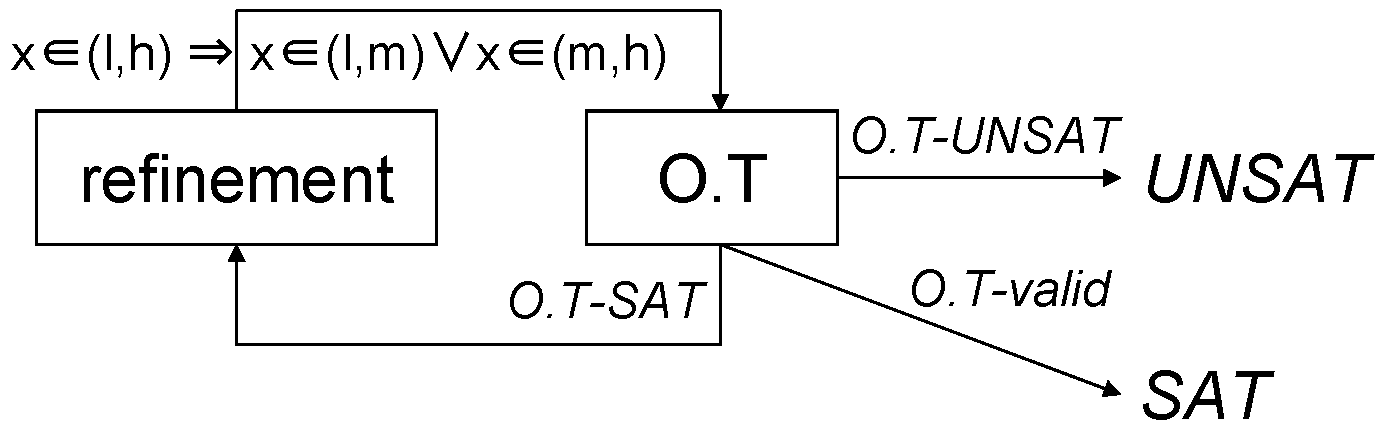
\includegraphics[height=0.6in,width=1.7in]{OTloop.png} & 
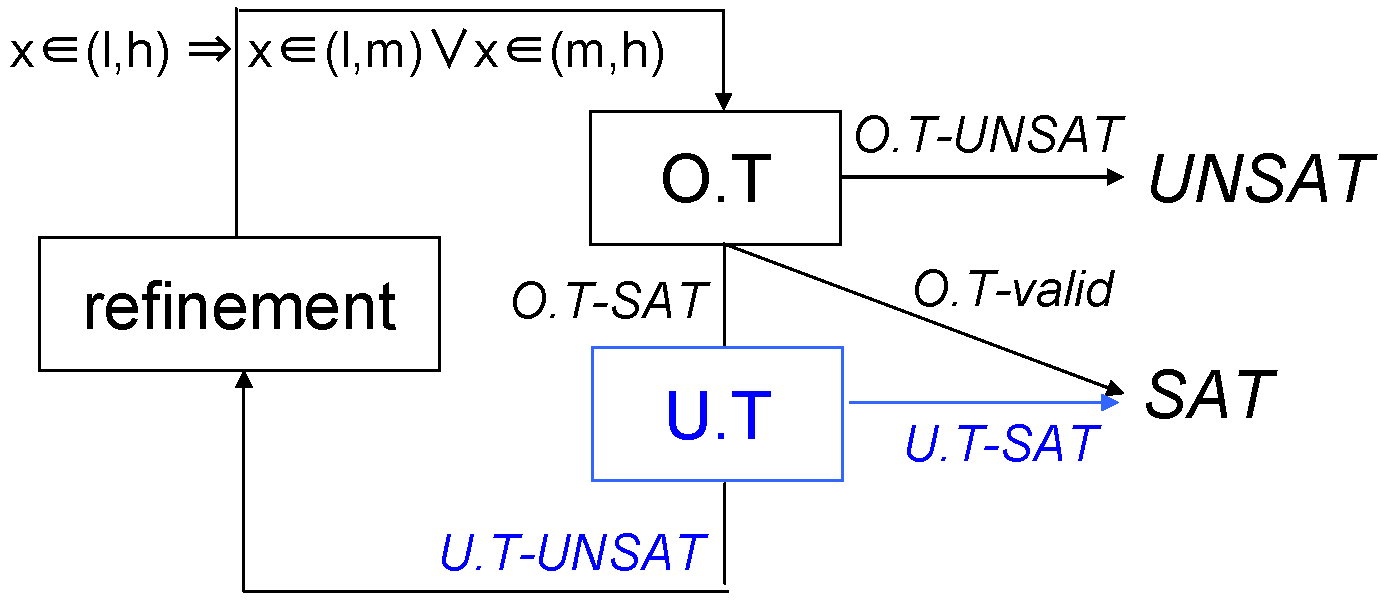
\includegraphics[height=0.9in,width=1.7in]{rasatloop.png} \\   
\mbox{(a) $O.T$ refinement loop} & \mbox{{\bf raSAT} loop} \\
\end{tabular}
\end{minipage} 
\caption{Rfinement loops} 
\label{fig:OTrefine} 
\end{figure}


\begin{definition} 
Let
$F = \exists x_1 \in I_1 \cdots x_n \in I_n. \bigwedge \limits_{j=1}^m f_j > 0$
for $I_i = (a_i,b_i)$.
A refinement strategy is {\em fair}, if, for each $c_j \in (a_j,b_j)$ and $\gamma > 0$, 
a decomposition of $I_i$ for each $i$ eventually occurs in $(c_j - \gamma, c_j + \gamma)$ 
(as long as neither SAT nor UNSAT is detected). 
\end{definition}

\begin{theorem} \label{th:RelComp}
Let
$F = \exists x_1 \in I_1 \cdots x_n \in I_n. \bigwedge \limits_{j=1}^m f_j > 0$
for $I_i = (a_i,b_i)$.
Assume that an over-approximation theory $O.T$ is converging, 
each $(a_i,b_i)$ is bounded, and a refinement strategy is fair. 
Then, 
\begin{itemize}
\item if $\exists x_1 \in (a_1,b_1) \cdots x_n \in (a_n,b_n) . \wedge_{i} f_i > 0$ is SAT, 
$O.T$ refinemnet loop eventually detects it, and
\item if $\exists x_1 \in [a_1,b_1] \cdots x_n \in [a_n,b_n] . \wedge_{i} f_i \geq 0$ is UNSAT, 
$O.T$ refinement loop eventually detects it.  
\end{itemize}
\end{theorem}


\begin{proof} 
The former is proved by the fact that, if $F$ is SAT, there exists a non-empty neiborhood (open box) 
in $\cap~\mathbb{S}(f_j)$. 
If the box decomposition strategy is fair, the refinemnet will eventually find such an open box. 

For the latter, assume that 
$\overline{F} = \exists x_1 \in [a_1,b_1] \cdots x_n \in [a_n,b_n] . \wedge_{i} f_i \geq 0$ is UNSAT. 
Thus, $\cap~\overline{\mathbb{S}(f_i)} = \emptyset$. 
Let $\delta_{j,k} = min \{|f_j(\bar{x}) - f_k(\bar{x})| \mid \bar{x} \in I_1 \times \cdots \times I_n\}$. 
Since $f_i$'s are continuous and $\overline{I_i}$'s are compact, $\delta_{j,k}$ is well defined,
and $\delta_{j.k} > 0$ for some $j,k$. 
Let $\delta = \frac{min \{ \delta_{j,k} \}}{2}$. 
Since $O.T$ is converging, there exists $\gamma > 0$ for $\delta > 0$ 
satisfying Definition~\ref{def:completeOT}, and fair decomposition eventually finds open boxes
such that $\mathbb{S}(f_j)$ and $\mathbb{S}(f_k)$ are separated. 
%\qed
\end{proof}

Limitations for detecting UNSAT occur on \emph{kissing} and \emph{convergent} cases. 
Fig.~\ref{fig:limit} left shows a kissing case 
$x^2 + y^2 < 2^2 \wedge (x-4)^2 + (y-3)^2 < 3^2$ such that 
$\overline{\mathbb{S}(- x^2 - y^2 + 2^2)} \cap \overline{\mathbb{S}(- (x-4)^2 - (y-3)^2 + 3^2)} 
= \{(x,y) \mid (1.6, 1.2)\}$. 
Thus, there are no coverings to separate them. 
%$x^2 + y^2 < 2^2$ and $(x-4)^2 + (y-3)^2 < 3^2$. 
%
Fig. \ref{fig:limit} right shows a convergent case 
$y > x + \frac{1}{x} \wedge y < x \wedge x > 0$, which is equivalent to 
$xy > x^2 + x \wedge y < x \wedge x > 0$. 
%The open box is $(0,\infty) \times (0,\infty)$ and 
There are no finite coverings to separate them. 
%$y > x + \frac{1}{x}$ and $y < x$ for $x > 0$. 

\begin{figure}[ht]
%\begin{minipage}[b]{1.0\linewidth}
\centering
\begin{tabular}{cc}
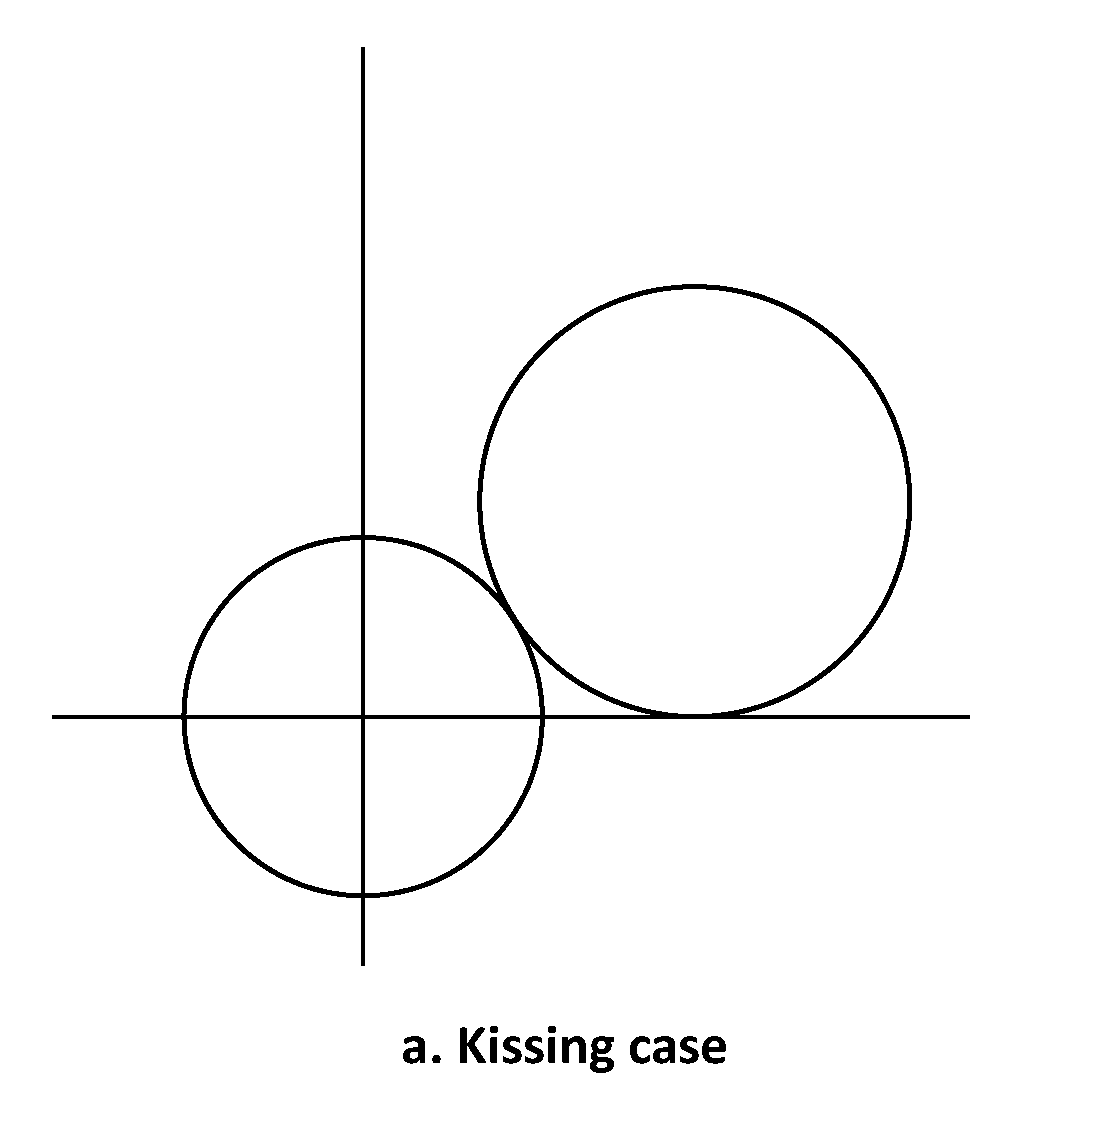
\includegraphics[height=1.65in,width=1.7in]{kissing.eps} &
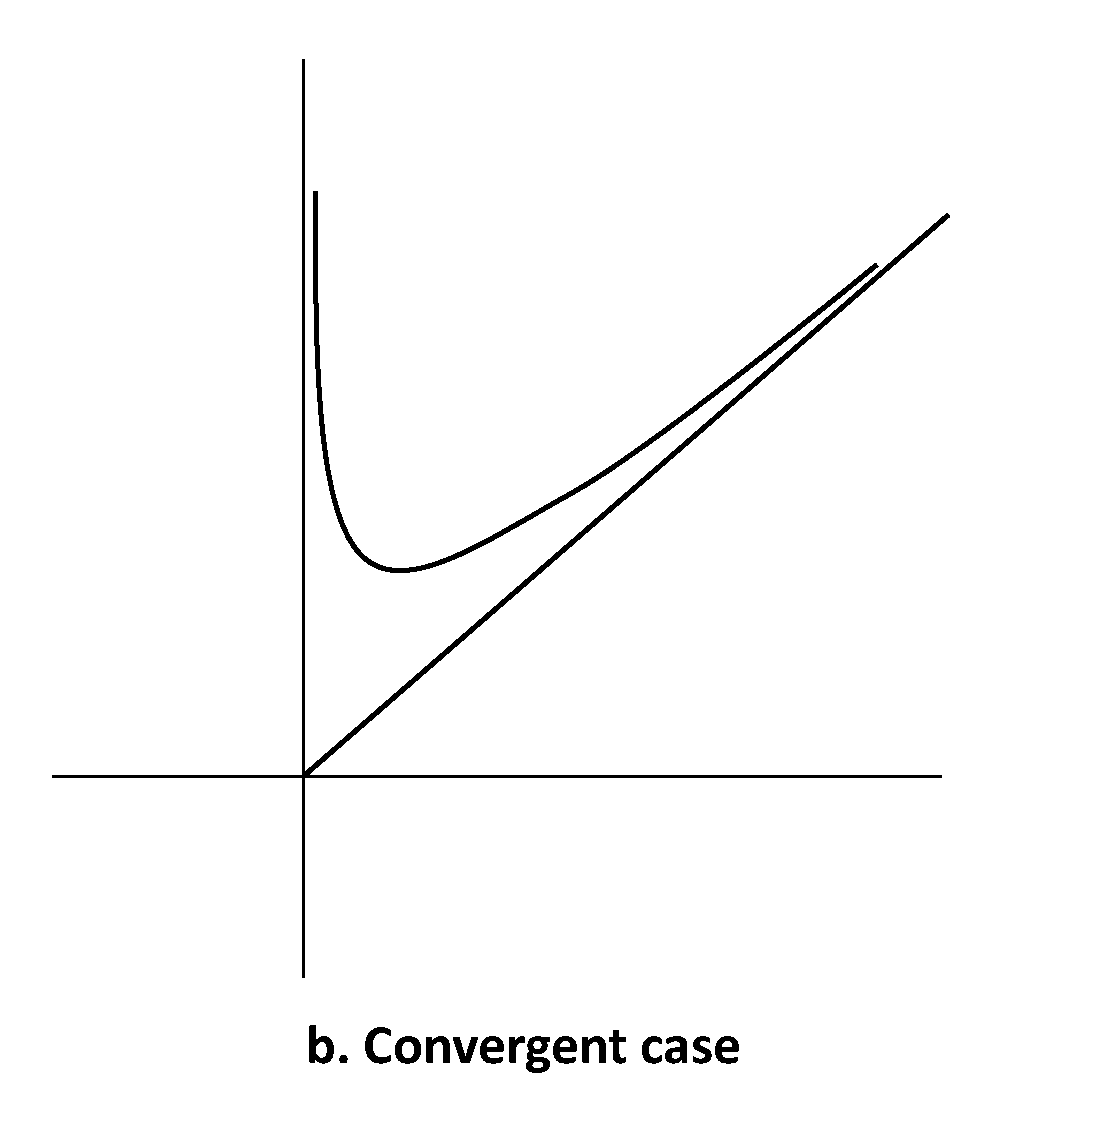
\includegraphics[height=1.65in,width=1.7in]{convergence.eps}
\end{tabular}
\caption{Limitations for proving UNSAT} 
\label{fig:limit} 
%\end{minipage}
\end{figure} 
\end{comment}